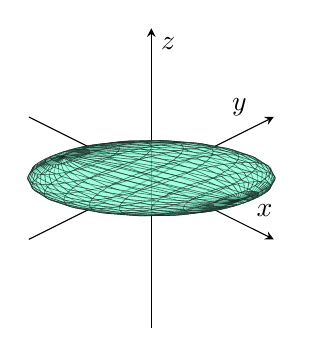
\begin{tikzpicture}
    \begin{axis}[%
        axis equal,
        width=8.5cm,
        height=8.5cm,
        colormap/blackwhite,
        axis lines = center,
        xlabel = {$x$},
        ylabel = {$y$},
        zlabel = {$z$},
        ticks=none, 
        enlargelimits=0.3,
        view/h=45,
        scale uniformly strategy=units only,
        zmin=-0.1,
        zmax=0.1,
        xmin=-3.5,
        xmax=3.5,
        ymin=-3.5,
        ymax=3.5,
        zmin=-3.5, 
        zmax=3.5
    ]
    \addplot3[%
        opacity = 0.5,
        surf,
        line width=0.2pt,
        fill=Aquamarine,
        point meta=100,
        z buffer = sort,
        samples = 25,
        variable = \u,
        variable y = \v,
        domain = 0:180,
        y domain = 0:360,
    ]
    (
        {4/2*cos(u)*sin(v) + 4/2*cos(v) -cos(u)*sin(v) - sin(u)*sin(v) + cos(v) }, 
        {4/2*cos(u)*sin(v) + 4/2*cos(v) +cos(u)*sin(v) +sin(u)*sin(v) -cos(v)}, 
        {0} 
    );
    \end{axis}
\end{tikzpicture}